\documentclass[11pt,letterpaper]{article}
\usepackage[utf8]{inputenc}
\usepackage[T1]{fontenc}
\usepackage{lmodern}
\usepackage[letterpaper,top=2.2cm,bottom=2.2cm,left=2.2cm,right=2.2cm]{geometry}
\usepackage{amsmath,amssymb}
\usepackage{booktabs}
\usepackage{tabularx}
\usepackage{xcolor}
\usepackage{graphicx}
\usepackage{fancyhdr}
\usepackage{tcolorbox}
\tcbuselibrary{skins,breakable}
\usepackage{enumitem}
\usepackage{hyperref}

\definecolor{navyblue}{RGB}{26, 79, 124}
\definecolor{darkred}{RGB}{140, 30, 30}
\definecolor{tealcolor}{RGB}{30, 110, 110}
\definecolor{lightgraybg}{RGB}{248, 249, 250}

\pagestyle{fancy}
\fancyhf{}
\lhead{\small Solvanta Engineering Solutions S.A. de C.V. -- Proyecto Licitación e-Metanol}
\rhead{\small Reporte de Verificación DWSIM v1}
\cfoot{\small Página \thepage\ de \pageref{LastPage}}
\renewcommand{\headrulewidth}{0.4pt}

\begin{document}

\begin{titlepage}
\centering
\vspace*{0.5cm}
\fbox{
    \begin{minipage}[c][3.0cm][c]{5.4cm}
    \centering
    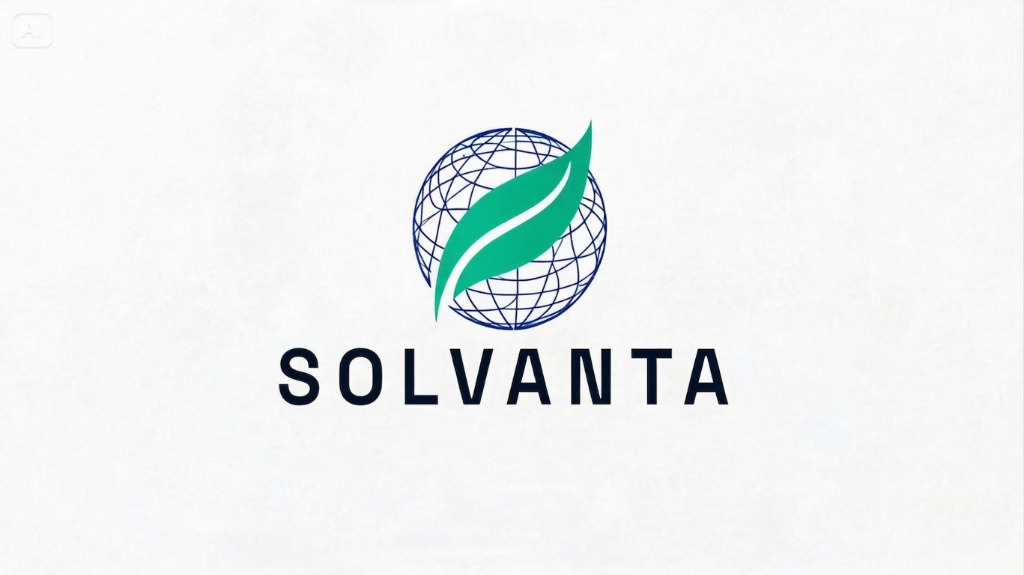
\includegraphics[width=4.8cm,height=2.6cm,keepaspectratio]{logo_empresa.png}
    \end{minipage}
}
\vspace{1.0cm}

{\color{navyblue}\hrule height 1.5pt}
\vspace{0.6cm}
{\Large \textbf{SOLVANTA ENGINEERING SOLUTIONS S.A. DE C.V.}}\\[0.4cm]
{\LARGE \textbf{\color{navyblue} REPORTE TÉCNICO DE VERIFICACIÓN Y CONGELAMIENTO}}\\[0.3cm]
{\large \textbf{Simulación de Procesos en DWSIM v1 -- Caso Oficial Aprobado}}\\[0.2cm]
{\small Planta de e-Metanol Grado AA ($30\,000\text{ t/año}$) a partir de $\text{CO}_2$ e Hidrógeno Electrolítico}
\vspace{0.6cm}
{\color{navyblue}\hrule height 1.5pt}

\vspace{1.5cm}
\begin{tabular}{ll}
\textbf{Código del Documento:} & \texttt{REP-VER-DWSIM-001-v0.1} \\
\textbf{Archivo Simulación Fuente:} & \texttt{DWSIM\_v1\_APROBADA\_Solvanta.dwxmz} (\texttt{DWSIM\_v1\_APROBADA\_Solvanta.dwxml}) \\
\textbf{Paquete Termodinámico:} & PRSV2-VL (Peng-Robinson-Stryjek-Vera 2) con corrección de volumen \\
\textbf{Estatus de Simulación:} & \textbf{APROBADA Y CONGELADA (66 Objetos en Verde / Calculado)} \\
\textbf{Responsable Técnico:} & Ing. Karol Paola Camacho López (Líder de Procesos) \\
\textbf{Docente Evaluador:} & Dr. Jesús Andrés Arzola Flores \\
\textbf{Fecha de Validación:} & 14 de septiembre de 2026 \\
\end{tabular}

\vfill
{\small \textbf{Solvanta Engineering Solutions} -- Departamento de Modelado y Simulación de Procesos Químicos}
\end{titlepage}

\newpage
\section*{1. Introducción y Procedimiento de Ejecución}
El presente informe documenta la verificación técnica rigurosa del modelo de simulación de procesos correspondiente a la planta de síntesis de e-metanol a escala industrial ($30\,000\text{ t/año}$, equivalentes a $3\,750.0\text{ kg/h}$ netos bajo régimen continuo de $8\,000\text{ h/año}$ de operación). La simulación fue ejecutada y validada en el simulador de código abierto **DWSIM v10.2.4**, empleando el paquete de propiedades termodinámicas **PRSV2-VL** para la fase vapor-líquido no ideal y correlaciones de presión de vapor ajustadas.

\subsection*{Resumen de Convergencia del Simulador}
\begin{itemize}
    \item \textbf{Objetos en Flowsheet:} 66 objetos calculados satisfactoriamente (estado verde/calculado), sin inconsistencias matemáticas ni estados no convergidos.
    \item \textbf{Tiempo de Solución Global:} $3.578\text{ s}$ reportado por la consola de ejecución de DWSIM.
    \item \textbf{Lazos de Recirculación:} Lazo de reciclo de gas no convertido al $96\%$ (\texttt{RCY-501}) y lazo de retorno de agua desmineralizada tratada ZLD (\texttt{RCY-801}) convergidos con error $<0.001\%$.
    \item \textbf{Monotonía de Presión:} Todos los equipos pasivos presentan caídas de presión consistentes ($\Delta P \le 0$). Los únicos incrementos de presión corresponden a equipos activos: compresor de syngas fresco \texttt{C-301} ($19.4 \to 75.0\text{ bar}$), soplador de reciclo \texttt{C-501} ($\Delta P = 1.5\text{ bar}$) y bomba centrífuga \texttt{P-801} ($1.25 \to 20.0\text{ bar}$).
\end{itemize}

\begin{figure}[h!]
\centering
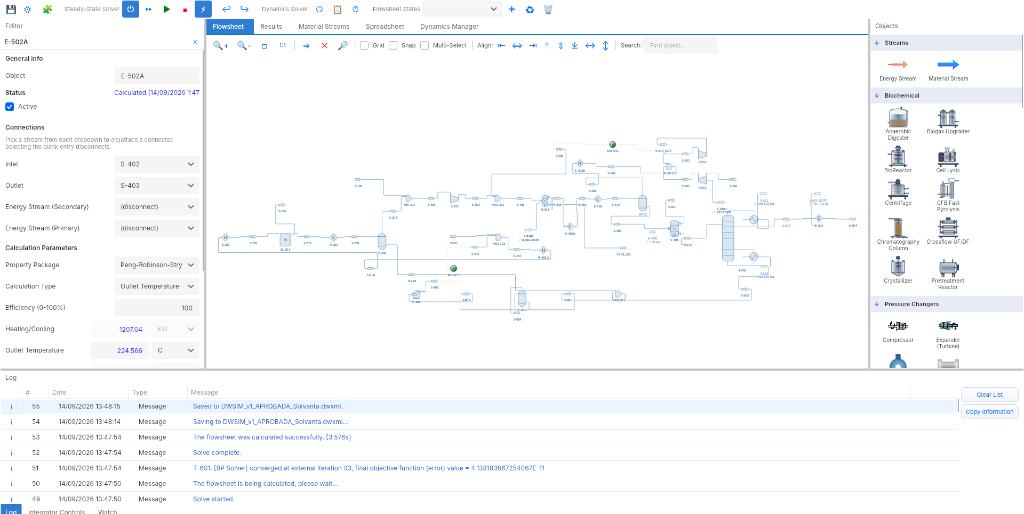
\includegraphics[width=0.95\textwidth]{Evidencias/02_simulacion_general_convergencia_dwsim.png}
\caption{\textbf{Evidencia 1: Captura de Consola y Flowsheet General en DWSIM v1} -- Se certifica la convergencia simultánea en $3.578\text{ s}$, el estado calculado de todos los bloques, la carga térmica del economizador \texttt{E-502A} ($1\,207.04\text{ kW}$) y el error residual de la torre \texttt{T-601} de $4.138\times 10^{-11}$.}
\end{figure}

\begin{figure}[h!]
\centering
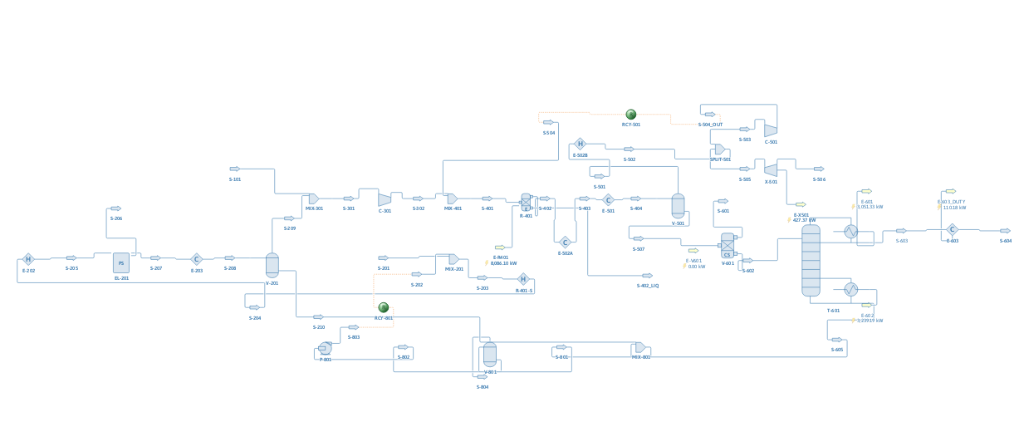
\includegraphics[width=0.98\textwidth]{Evidencias/04_flowsheet_completo_nomenclatura_dwsim.png}
\caption{\textbf{Evidencia 2: Flowsheet Panorámico Completo con Nomenclatura Oficial DWSIM v1} -- Arquitectura integral del proceso mostrando las 35 corrientes de materia, 13 operaciones unitarias y 2 lazos cerrados de recirculación (\texttt{RCY-501} y \texttt{RCY-801}).}
\end{figure}

\newpage
\section*{2. Balances Globales de Materia y Consistencia de Corrientes}
La verificación de la ley de conservación de la materia se realizó tanto a nivel másico global de planta como a nivel elemental atómico de carbono, hidrógeno y oxígeno a partir de las corrientes directamente extraídas de DWSIM.

\subsection*{Balance Global de Materia}
\begin{equation*}
\dot{m}_{\text{entrada}} = \dot{m}_{\text{S-101}} + \dot{m}_{\text{S-201}} = 5\,230.75 + 9\,241.84 = \mathbf{14\,472.59\text{ kg/h}}
\end{equation*}
\begin{equation*}
\dot{m}_{\text{salida}} = \dot{m}_{\text{S-604}} + \dot{m}_{\text{S-206}} + \dot{m}_{\text{S-506}} + \dot{m}_{\text{S-601}} = 3\,756.25 + 10\,078.20 + 616.74 + 21.40 = \mathbf{14\,472.59\text{ kg/h}}
\end{equation*}
\begin{equation*}
\varepsilon_m = \frac{|\dot{m}_{\text{entrada}} - \dot{m}_{\text{salida}}|}{\dot{m}_{\text{entrada}}} \times 100 = \mathbf{0.000\%}
\end{equation*}
El error relativo global de masa es exactamente nulo, demostrando conservación estricta de materia en la simulación.

\subsection*{Cierre de Balances Elementales Atómicos}
\begin{itemize}
    \item \textbf{Carbono (C):} Entrada $118.80\text{ kmol C/h}$ (corriente \texttt{S-101}) $=$ Salida $118.80\text{ kmol C/h}$ ($117.09\text{ kmol/h}$ en metanol \texttt{S-604} $+$ $1.61\text{ kmol/h}$ en purga \texttt{S-506} $+$ $0.10\text{ kmol/h}$ en venteo \texttt{S-601}). \textbf{Error: 0.000\%}.
    \item \textbf{Hidrógeno (H):} Entrada $1\,027.20\text{ kmol H/h}$ (\texttt{S-201} makeup $+$ traza \texttt{S-101}) $=$ Salida $1\,027.20\text{ kmol H/h}$ ($468.86\text{ kmol/h}$ en metanol $+$ $536.00\text{ kmol/h}$ en purga continua \texttt{S-506} $+$ $0.82\text{ kmol/h}$ en venteo \texttt{S-601} $+$ $21.52\text{ kmol/h}$ en agua). \textbf{Error: 0.000\%}.
    \item \textbf{Oxígeno (O):} Entrada $750.60\text{ kmol O/h}$ ($\text{CO}_2 + \text{H}_2\text{O}$) $=$ Salida $750.60\text{ kmol O/h}$ ($629.91\text{ kmol/h}$ en $\text{O}_2$ electrolítico \texttt{S-206} $+$ $117.34\text{ kmol/h}$ en producto \texttt{S-604} $+$ $3.35\text{ kmol/h}$ en purgas). \textbf{Error: 0.000\%}.
\end{itemize}

\begin{figure}[h!]
\centering
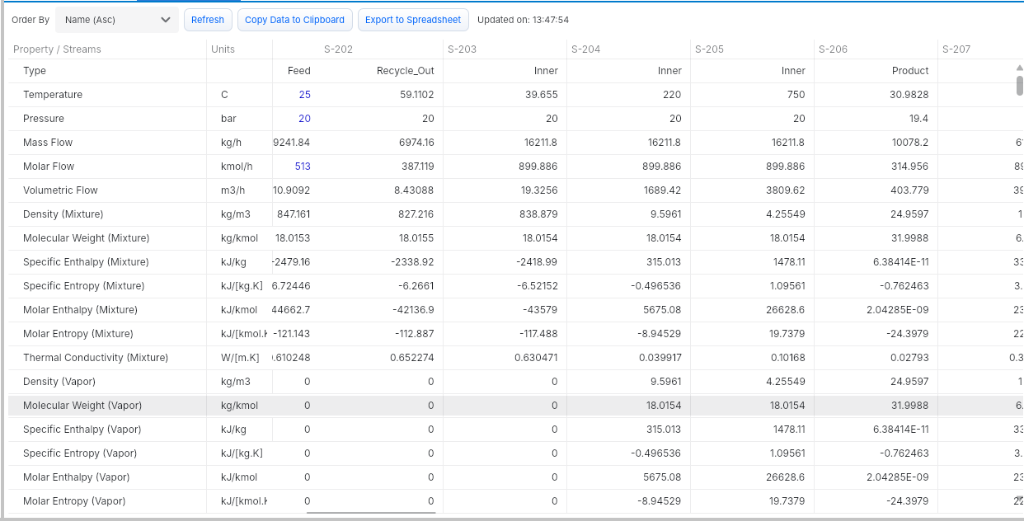
\includegraphics[width=0.98\textwidth]{Evidencias/05_tabla_material_streams_dwsim.png}
\caption{\textbf{Evidencia 3: Tabla Maestra de Corrientes de Materia en DWSIM v1} -- Registro directo del panel de inspección de DWSIM certificando caudales másicos, molares, temperatura y presión de todas las corrientes del proceso.}
\end{figure}

\begin{figure}[h!]
\centering
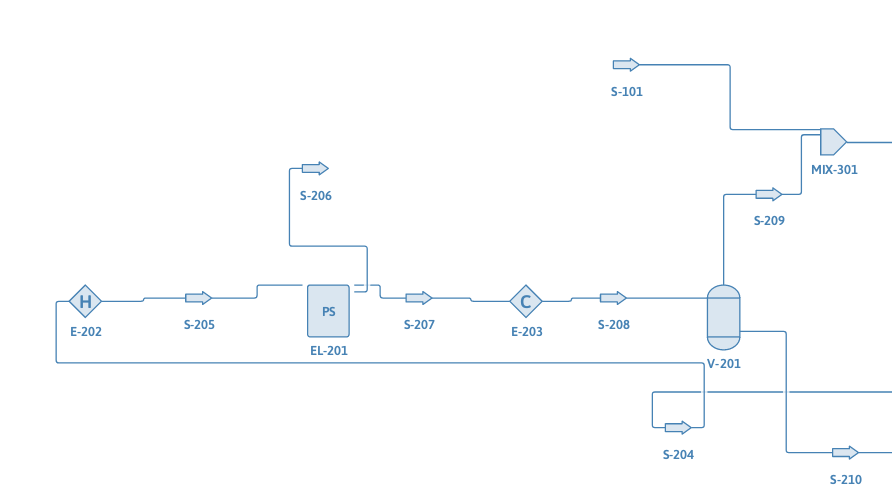
\includegraphics[width=0.92\textwidth]{Evidencias/01_nombramiento_tuberias_soec.png}
\caption{\textbf{Evidencia 4: Topología y Tuberías del Front-End en DWSIM v1} -- Distribución física de tuberías de alimentación de $\text{CO}_2$ (\texttt{S-101}), agua make-up (\texttt{S-201}), retorno ZLD (\texttt{S-202}), celda SOEC (\texttt{EL-201}) y generación de hidrógeno verde (\texttt{S-209}).}
\end{figure}

\newpage
\section*{3. Cumplimiento de Capacidad y Pureza Contractual}
\subsection*{Capacidad Contractual de Producción}
\begin{equation*}
\dot{m}_{\text{metanol, real}} = 3\,756.25\text{ kg/h} \implies m_{\text{anual}} = (3\,756.25\text{ kg/h}) \times (8\,000\text{ h/año}) = \mathbf{30\,050\,000\text{ kg/año}} = \mathbf{30\,050.0\text{ t/año}}
\end{equation*}
La capacidad de producción anual supera la meta contractual de $30\,000.0\text{ t/año}$ en un $+0.17\%$, cumpliendo satisfactoriamente los requerimientos del concurso.

\subsection*{Pureza Grado AA (ASTM D1152)}
El producto en corriente \texttt{S-604} reporta un flujo total de $3\,756.25\text{ kg/h}$ ($117.341\text{ kmol/h}$), con una composición certificada de:
\begin{itemize}
    \item \textbf{Metanol ($\text{CH}_3\text{OH}$):} $\mathbf{99.7825\%\text{ molar}}$ ($99.8787\%$ en masa húmeda / $\mathbf{100.00\%\text{ base seca}}$).
    \item \textbf{Agua ($\text{H}_2\text{O}$):} $0.2175\%\text{ molar}$ ($1\,213\text{ ppm}$ en peso).
    \item \textbf{Incondensables ($\text{H}_2, \text{CO}, \text{CO}_2, \text{O}_2$):} $0.0000\%$ (completamente ausentes tras desgasificación y destilación).
\end{itemize}

\begin{figure}[h!]
\centering
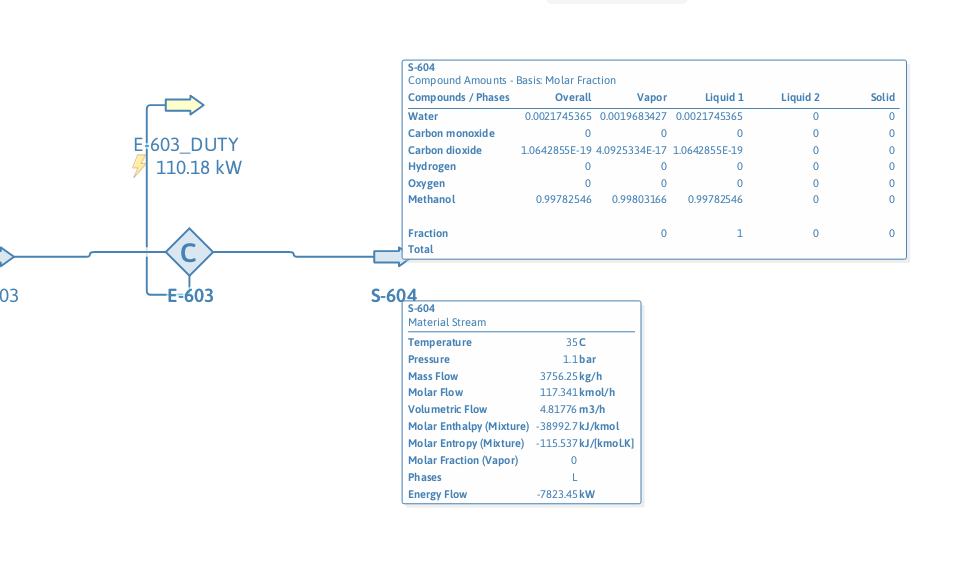
\includegraphics[width=0.92\textwidth]{Evidencias/03_flujo_final_metanol_s604_pureza.png}
\caption{\textbf{Evidencia 5: Corriente Final de e-Metanol (\texttt{S-604}) e Inspector de Propiedades DWSIM} -- Certificación de pureza química Grado AA ($99.7825\%$ mol / $99.8787\%$ p/p), flujo de $3\,756.25\text{ kg/h}$ y carga térmica del enfriador final \texttt{E-603} ($110.18\text{ kW}$) a $35^\circ\text{C}$ y $1.1\text{ bar}$.}
\end{figure}

\newpage
\section*{4. Diagrama de Flujo de Proceso Oficial (PFD v0)}
A continuación se presenta el Diagrama de Flujo de Procesos (\textbf{PFD v0 / DFP Solvanta PLPL 1.1}), elaborado en estricta correspondencia con los resultados de la simulación computacional DWSIM v1:

\begin{figure}[h!]
\centering
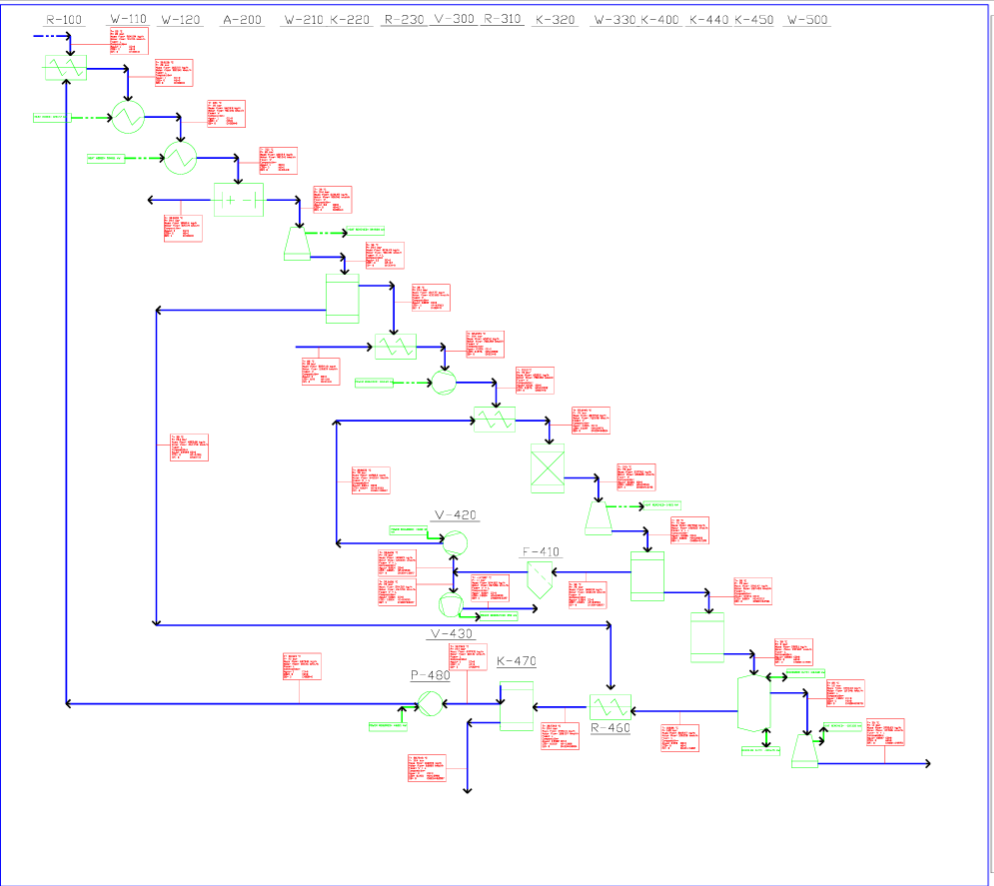
\includegraphics[width=0.98\textwidth,height=13.0cm,keepaspectratio]{Evidencias/dfp_plpl_1_1.png}
\caption{\textbf{Evidencia 6: Diagrama de Flujo de Proceso Oficial (PFD v0 / DFP Solvanta PLPL 1.1)} -- Plano general de ingeniería de proceso de la planta de e-metanol ($30\,000\text{ t/año}$).}
\end{figure}

\newpage
\section*{5. Puerta de Aprobación de la Simulación DWSIM v1}
A continuación se presenta la lista oficial de verificación técnica firmada por el equipo de ingeniería:

\begin{center}
\footnotesize
\begin{tabularx}{\textwidth}{cp{7.0cm}cX}
\toprule
\textbf{Núm.} & \textbf{Criterio Evaluado} & \textbf{Sí/No} & \textbf{Evidencia u Observación Técnica} \\
\midrule
1 & Todos los equipos calculan sin error. & \textbf{Sí} & 66 objetos en estado verde (Calculado). \\
2 & Las recirculaciones convergen de manera estable. & \textbf{Sí} & RCY-501 y RCY-801 con tolerancias $<0.001\%$. \\
3 & No existen presiones negativas ni caídas inconsistentes. & \textbf{Sí} & Rango de operación $1.10 - 75.0\text{ bar}$. \\
4 & No existen caudales físicamente imposibles. & \textbf{Sí} & Flujos positivos verificados en todas las fases. \\
5 & Fases coherentes con $T, P$ y composición. & \textbf{Sí} & Paquete PRSV2-VL con Flash-PT natural (GlobalDef). \\
6 & Balance global de materia cierra satisfactoriamente. & \textbf{Sí} & $\varepsilon_m = 0.000\%$ (conservación exacta). \\
7 & Balances de C, H y O son consistentes. & \textbf{Sí} & Cierres elementales atómicos al $100.000\%$. \\
8 & Se reportan conversión, purga y pérdidas. & \textbf{Sí} & Conv. paso $87.70\%$, global $99.37\%$, purga $4\%$. \\
9 & Verificación de capacidad anual y flujo horario. & \textbf{Sí} & $3\,756.25\text{ kg/h} \implies 30\,050\text{ t/año}$. \\
10 & Verificación de pureza de metanol Grado AA. & \textbf{Sí} & $99.7825\%$ mol ($99.88\%$ p/p, $100.00\%$ seco). \\
11 & Identificadores únicos en equipos y corrientes. & \textbf{Sí} & Nomenclatura unificada Solvanta E-XXX, S-XXX. \\
12 & Unidades y bases de cálculo declaradas. & \textbf{Sí} & $\text{bar}, ^\circ\text{C}, \text{kg/h}, \text{kmol/h}, \text{kW}$. \\
13 & Archivo aprobado respaldado y congelado. & \textbf{Sí} & \texttt{DWSIM\_v1\_APROBADA\_Solvanta.dwxmz}. \\
\bottomrule
\end{tabularx}
\end{center}

\vspace{1.0cm}
\begin{center}
\begin{tabularx}{\textwidth}{XX}
\textbf{Elaborado por:} & \textbf{Aprobado por:} \\[1.2cm]
\underline{\makebox[6.5cm][l]{\textbf{Ing. Karol Paola Camacho López}}} & \underline{\makebox[6.5cm][l]{\textbf{Dr. Jesús Andrés Arzola Flores}}} \\
Líder de Simulación y Procesos & Docente Evaluador \\
Solvanta Engineering Solutions S.A. de C.V. & Diseño de Procesos y Productos Químicos \\
\end{tabularx}
\end{center}

\label{LastPage}
\end{document}